\documentclass[12pt, letterpaper]{article}
\usepackage{graphicx}
\title{Error Detection and Corrective Feedback using Anomaly Detection in Long Jump Athletes}
\author{Pradyumn Vikram}
\begin{document}
\maketitle

\tableofcontents

\begin{abstract}
This report provides a descriptive analysis of the process undertaken in building Project Kitty
 - An analytics module developed to detect and provide corrective feedback to long jump athletes using
 video footage. 
\end{abstract}

\section{Choice of Sport and Rationale}

Long jump has long been a beloved athletic sport, with players from 60+ countries
taking part in the Olympics for long jumping. Keeping aside it's popularity, it is 
also a highly technical sport, requiring technique and skill. Correction in posture
as well as general approach to the sport if optimised, can help an athlete improve his/her
 performance by a large margin. We have focused on various factors playing a vital role 
 in the distance covered by an athlete during a long jump such as - 
 \begin{itemize}
    \item Hip flexion
    \item Knee flexion
    \item Trunk angle
    \item Run-up velocity
 \end{itemize}
 The project aims to provide descriptive feedback 
 on the above mentioned factors to an athlete. The factors to evaluate have been
 chosen by referring to online sources on biomechanics.

 \section{Data Collection and Extraction of Long Jump Clips from Extended Videos}
I have used the YouTubeDL and youtubesearch module to extract feed from
the Olympic games of four different years - Beijing, Rio, Tokyo and Paris.
The extracted videos being very large in size for preprocessing have been split
into smaller segments of approximately 50mb in size using the ffmpeg module,
 for ease of processing and extracting segments.
 \\\\For extraction of segments of athletes performing long jumps, 
 I first manually cropped a singular reference video of an athlete performing 
 the movements (Run-up, Take-off, Flight and Landing). The goal is now to find timestamps
 in the game feed videos representing similar movement as in the reference video for which I attempted two approaches - 
 \begin{itemize}
    \item First, I tried to extract the perceptual hash of the reference video, 
    and compare it to fixed segments (frames) in the videos where I want to extract 
    clips from. However this approach did not work as - 
    \begin{itemize}
        \item The video files differed too much, due to differences in the track 
        along with visual differences in various aspects, such as jersey color etc.
        \item The visual summary generated (collage of images) could not capture the temporal data, 
        as well as the features needed to extract the requiered frames.
    \end{itemize}
    \item Second, I used the ResNet3D-18 pretrained CNN (trained on the Kinetics 400 dataset - comprising of data involving 
    human action classes). 
    \begin{itemize}
        \item Each video snippet was segmented in 16 frames - each of which was then standardised with the mean and standard deviation of the kinetics 400 dataset
        \item These frames were the stacked to form a tensor of shape [channel, frames, width, height], and then reshaped to [1, channel, frames, width, height] (this is required for input to the ResNet model)
        \item This was then passed into the stem layer and 4 residual blocks of the pre-trained residual network to extract features from temporal data
        \item Now we extract the mean of the frames, width and height column; flattening the array furthurmore, to represent the entire sequence in an array of 1 dimension (a vector)
        \item This was then compared using cosine similarity with the extracted 1 dimensional vector of the reference video
        \item Those scoring above a set threshold were flagged and then later joined with other segments who overlap to get a complete video clip
        \item These videos are then clipped according to the extracted timestamps, giving very accurate results
    \end{itemize}
    This approach, using the Residual Network returned very accurate clips of athletes performing long jumps, showing
    that the network managed to capture the temporal features very well. However not entirely immune to error, I had to iterate through all extracted clips and remove 15 out of 240 clips which did not contain the frames required
 \end{itemize}

 \section{Phase Segmentation of Long Jump Clips}

 Now that we have extracted clips of athletes performing long jumps and eliminated a majority of the noise
 in the form of commentator box frames, audience etc. We now attempt to divide the clip into phases for furthur analysis,
 namely - (Run up, Take off, Flight and Landing). Since I had no labelled data, clustering seemed to be the most appropriate approach.
I used mediapipe to extract features from each frame, which were then passed into the K-Means clustering algorithm to label each frame with an ID from 0 to 4.

The features extracted namely -
\begin{itemize}
    \item Hip Velocity in X
    \item Hip Velocity in Y
    \item Hip Y coordinate
    \item Trunk angle with the Z-axis
    \item Hip-knee angle
    \item Right knee angle
    \item Left Knee angle
    \item Lowest foot coordinate
\end{itemize}
were chosen so via online research and trial and error, the evolution of these features through-out the frames can be seen in Figure 1

\begin{figure}[htbp]
    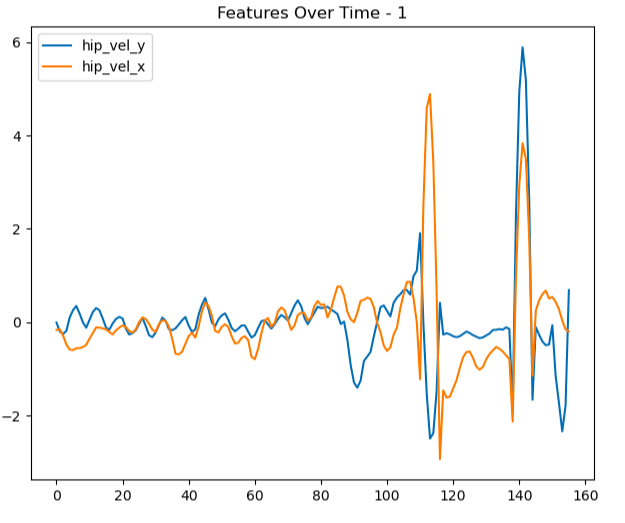
\includegraphics[width=0.5\textwidth]{plots/graph1.png}
    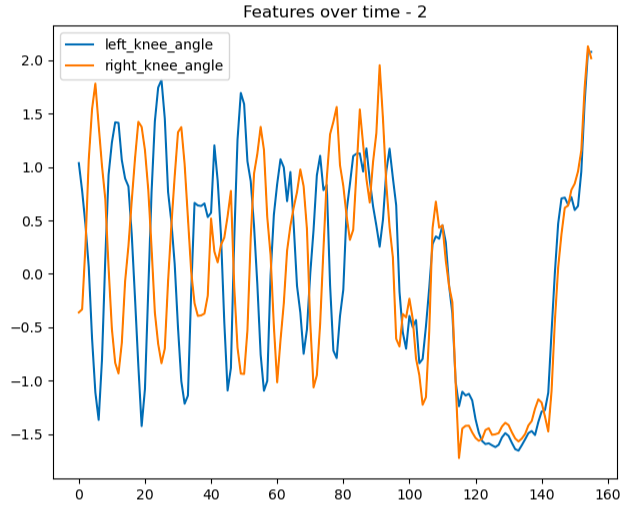
\includegraphics[width=0.5\textwidth]{plots/graph2.png}
    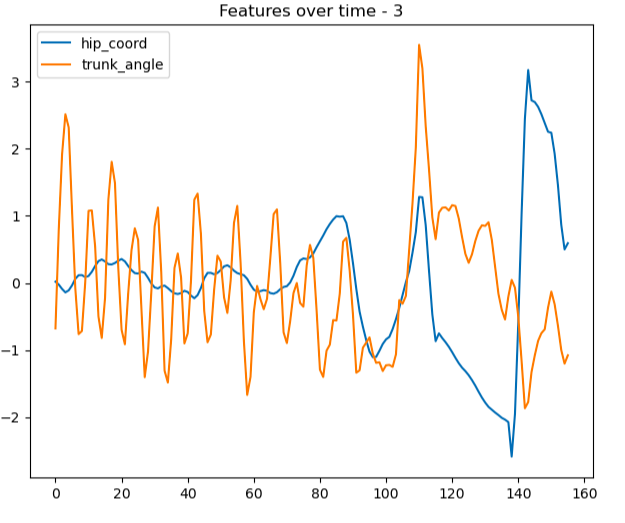
\includegraphics[width=0.5\textwidth]{plots/graph3.png}
    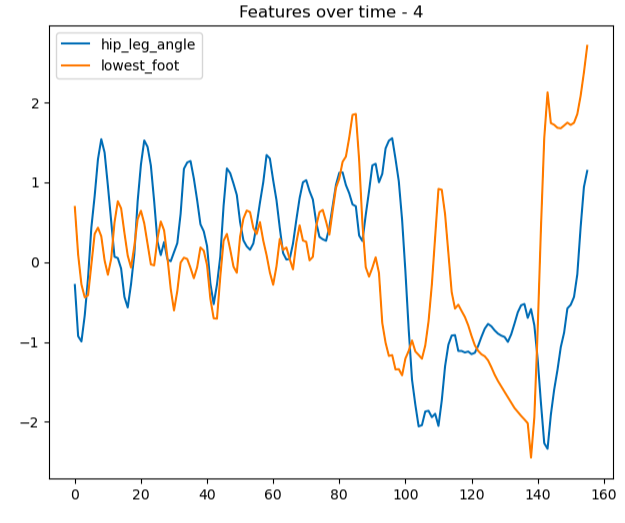
\includegraphics[width=0.5\textwidth]{plots/graph4.png}
    \caption{Evolution of Features over Frames}
\end{figure}
K-Means clustering was then employed after standardisation over all the features giving suitable output with some error.
The clusters were then smoothened by using the fact that one phase when completed cannot be repeated again, see Figure 2
\begin{figure}[htbp]
    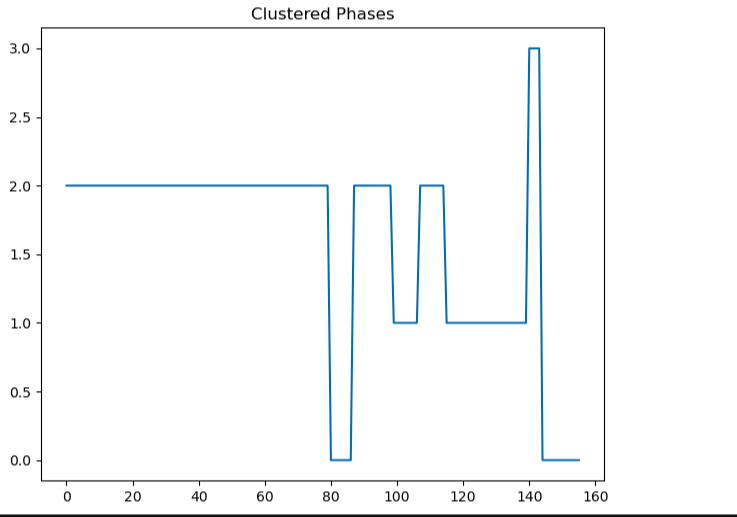
\includegraphics[width=0.5\textwidth]{plots/cluster_graph.png}
    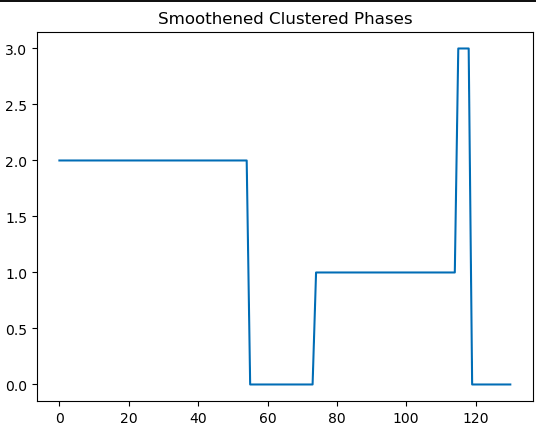
\includegraphics[width=0.5\textwidth]{plots/cluster_smooth.png}
    \caption{Clustered Frames - Before vs After smoothing}
    \label{fig:clustered}
\end{figure}

This clustering after employed on each frame, then enabled me to divide the phases into four datasets - corresponding to each phase.
These can now be used for anomaly detection and correction by engineering appropriate features.

\section{Anomaly Detection and Corrective Prediction}

For anomaly detection ie isolating out errors and providing descriptive corrective feedback, I considered using Isolation Forests or One Class SVMs.
Isolation Forests was ruled out since it would be difficult to identify which feature caused the anomaly and isolated the sample from the normal. I engineered
2 features each for each phase based on online research and prioritising important factors for good technique. Each data frame once standardised was then fit to a One Class SVM.
The decision function plotted can be reviewed in Figure 3

\begin{figure}[htbp]
    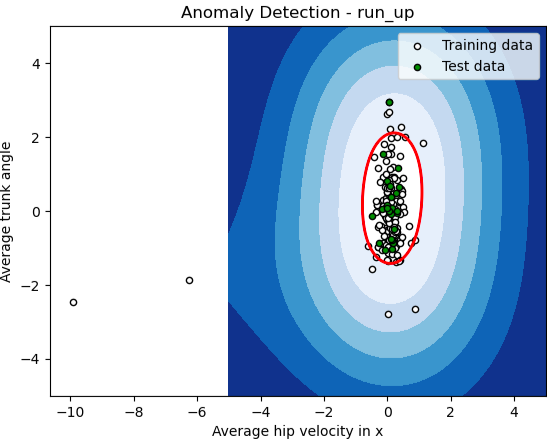
\includegraphics[width=0.5\textwidth]{plots/model_run_up.png}
    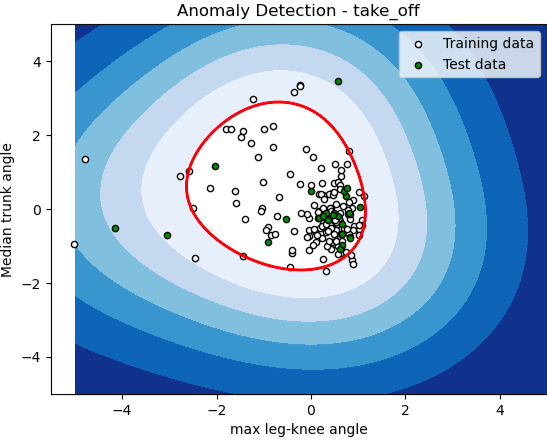
\includegraphics[width=0.5\textwidth]{plots/model_take_off.png}
    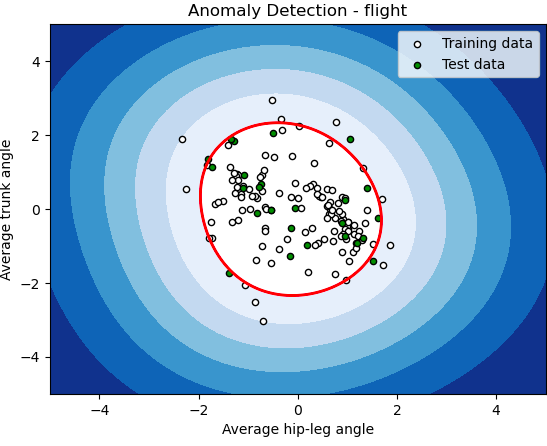
\includegraphics[width=0.5\textwidth]{plots/model_flight.png}
    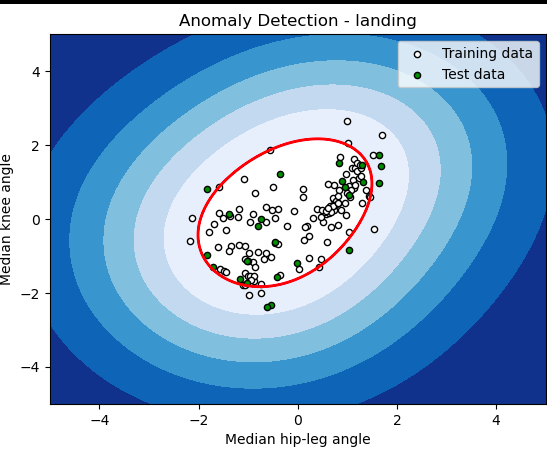
\includegraphics[width=0.5\textwidth]{plots/model_landing.png}
    \caption{Decision Boundaries - Showing model fit and performance}
\end{figure}

For providing descriptive feedback, I first identify outliers (any point not in the contour), then I evaluate it's x and y distance from the center of the contour. Since x and y represent the 2 features based on which the contour was made, whichever distance is greater tell me, what was the major contributor to the anomaly - something I cannot do with Isolation Forests. Then the feature contributing most to the anomaly is then acted upon to provide feedback to the athlete in four phases.

Proceeding to build the analytics module, I took an unseen data sample (Trimmed video of an athlete performing long jump from the Asian Games - refer to misc/), in which the model provided descriptive feedback. The interface for the module and the output can be seen in Figure 4

\begin{figure}[htbp]
    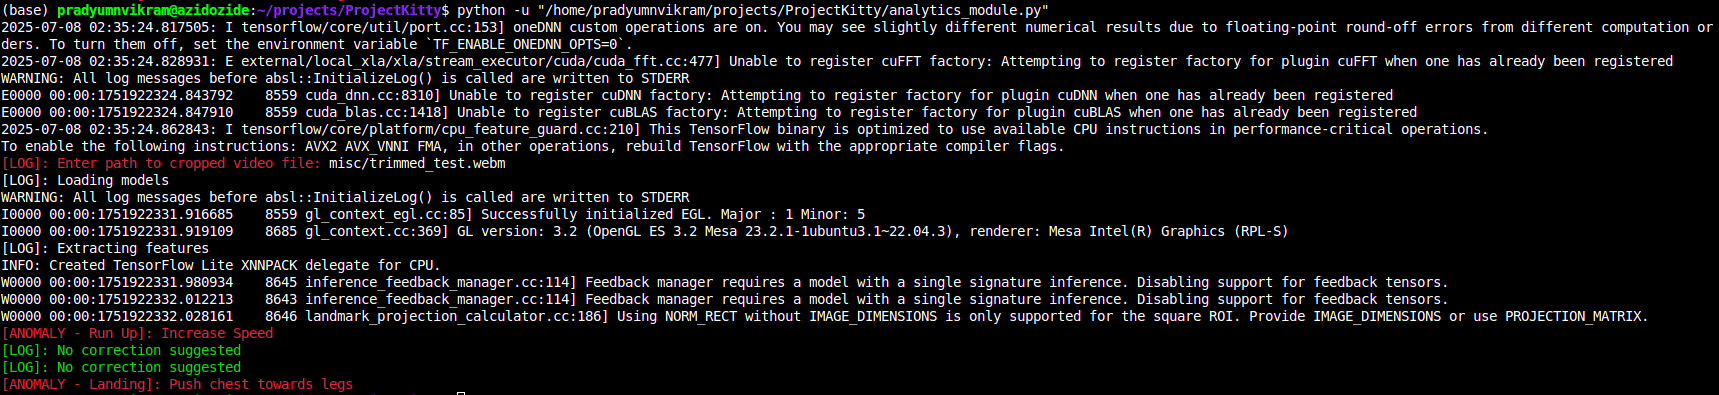
\includegraphics[width = 1.2\textwidth]{plots/result.png}
    \caption{Analytics module - UI and Test output}
\end{figure}

\section{Summary and Drawbacks}
We have developed a module which can evaluate long jumps and provide corrective feedback.
\begin{itemize}
    \item The pipeline is still sometimes struggling to cluster some video clips into various phases
    \item Since I have only unlabelled data, it is difficult to analyse the performance of the analytics module (The visualisation is my only source of verification)
    \item More features can be added for descriptive feedback - seeing how currently there are only 2 per phase
\end{itemize} 

\end{document}